\documentclass{tufte-handout}

%\geometry{showframe}% for debugging purposes -- displays the margins
\usepackage{pdfpages}
\usepackage{amsmath}
\usepackage{natbib}
\usepackage{booktabs}
\usepackage{multicol}
\usepackage[version=4]{mhchem} 

\bibfont{\small} % Doesn't see to work...
\usepackage{graphicx}

\setkeys{Gin}{width=\linewidth,totalheight=\textheight,keepaspectratio}
% \graphicspath{{graphics/}}

\newenvironment{itemize*}%
  {\begin{itemize}%
    \setlength{\itemsep}{0pt}%
    \setlength{\parskip}{0pt}}%
  {\end{itemize}}
	
\newenvironment{enumerate*}%
  {\begin{enumerate}%
    \setlength{\itemsep}{0pt}%
    \setlength{\parskip}{0pt}}%
  {\end{enumerate}}
	

\title{Particle Size Analysis of Soils by Sedimentation %\thanks{Isaac Medina}
}
\author[Marc Los Huertos]{Marc Los Huertos}
%\date{}  % if the \date{} command is left out, the current date will be used

% \SweaveOpts{prefix.string=graphics/plot} % Created a "graphics" subdirectory to 

\setsidenotefont{\color{blue}}

\usepackage{Sweave}
\begin{document}
\input{Soil_Texture_Analysis_160528-concordance}

\maketitle% this prints the handout title, author, and date
\begin{abstract}
\noindent Soil is usually composed of particles with a mix of sizes where the relative proportion of size classes define the soil texture. As a property of a soil, the texture can determine water relations, bio-availability of nutrients and toxics, and soil biogeochemistry. Soil texture can be determined using qualitative or quantitative methods that might be employed in the field or in the laboratory, respectively. While classes are distinguished in the field and the class is then used to determine crop suitability and to approximate the soils responses to environmental and management conditions such as drought, fertility, or calcium (lime) requirements.
\end{abstract}

%\printclassoptions

% Setting up the margins, etc for R

\section{Outline and Outcomes}
This handout describes how soil samples can be quantitatively analyzed using hydrometer to promote the following skills:

\begin{enumerate}
	\item Understand the equations that describe how particle size and the terminal velocity in a suspension;
	\item Use sedimentation methods to measure density changes in soil suspensions; and
	\item Apply equations to calculate the density and percent of a sample in suspension to calculate the particle sizes of a soil sample. 
\end{enumerate}

\section{Background}

Soils are composed of mineral particles, organic matter, water and air. In general, most of the mass of soil is composed of mineral particles and the size or texture of these particles influence a range of physical and biological processes in soil. In the simplest cases, we can categorize the size of particles into three groups: Sand, silt, and clay. In general, we consider soil to be made up of particles that can pass through a 2 mm sieve, aka No. 10 sieve (Figure \ref{fig:8stainless_sieve}). 

\begin{marginfigure}
	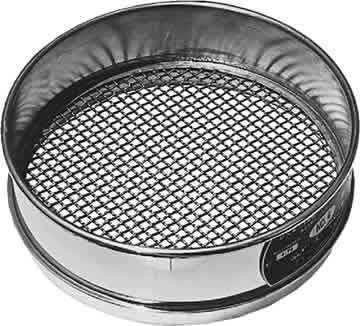
\includegraphics{8stainless_sieve.jpg}
	\caption{Sieves are circular dishes with a mesh bottom. Each sieve type have different mesh sizes, thus can be used to ``split'' soils based on the size of particles, where particles smaller than the mesh fall through and larger particles are retained.}
	\label{fig:8stainless_sieve}
\end{marginfigure}

\begin{table}
		\begin{tabular}{lrr}\hline
Classification 					&  USDA System 		& World Reference Base\\ \hline\hline
			Clay 							& <0.002 mm 			& <0.002 mm \\
			Silt 							& 0.002-0.05 mm 	& 0.002-0.063 mm\\
			Very fine sand		& 0.05-0.10 mm 		& 0.063-0.0125 mm\\
			Fine sand 				& 0.10-0.25 mm 		& 0.0125-0.20 mm\\
			Medium sand				& 0.25-0.50 mm 		& 0.20-0.63 mm\\
			Coarse sand 			& 0.50-1.00 mm 		& 0.63-1.25 mm\\
			Very coarse sand	& 1.00-2.00 mm 		& 1.25-2.00 mm\\
			Gravel 						& >2.0 mm 				& >2.0 mm \\ \hline
		\end{tabular}
\end{table}


There are a number of references that explain various methods to conduct a particle analysis, such as \citep{gee1986particle, day1965particle, beretta2014soil}. For our purpose, we will use the method developed by the ASTM International that capitalizes on the correlation between the size of particles, their terminal velocity, and the density of the suspension \citep{standard2007d422}. 

This handout describes how we can use a hydrometer to measure density of a soil suspension and how this density changes with time. As the density changes, we can use several equations to estimate the proportion of particle sizes. 

\begin{figure}
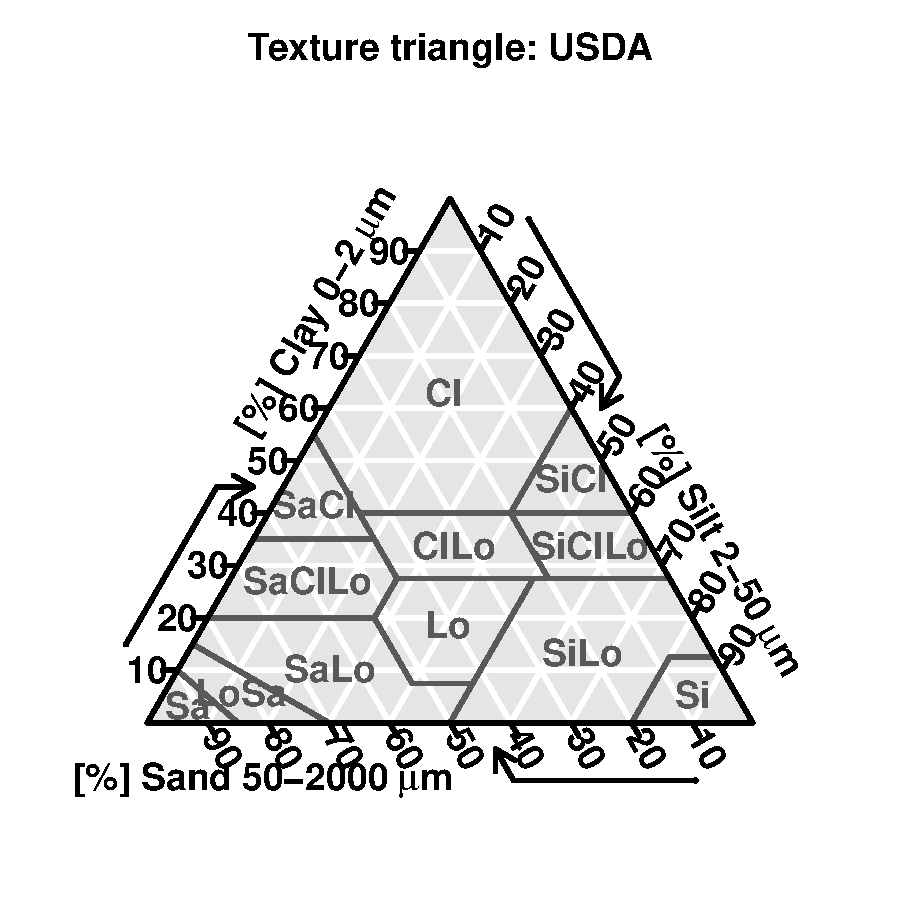
\includegraphics{Soil_Texture_Analysis_160528-USDATT}
\end{figure}

\subsection{Physics of Particles in Suspension}

The behavior of particles in a suspension is well understood\sidenote{This section is from \citet{hillel1998environmental}.}, where particles are accelerated by the force of gravity, g, which is 9.8 m/sec$^2$. Except in a vacuum, particles experience resistance. This force of resistance, $F_r$, is proportional to the radius and velocity of the particle and the viscosity of the fluid that surrounds it. This was defined by George Stokes in 1851 as

\begin{equation}\label{eq:Fr}
F_r = 6\pi \eta r \nu
\end{equation}

\noindent where r is the radius, 
$\eta$ is the fluid viscosity and 
$\nu$ is the velocity.

The downward force due to gravity, $F_g$, proportional to the volume of the particle, $(4/3)\pi r^3$, and difference in particle and fluid densities, $\rho_p - \rho_f$.\sidenote{suspension, solid, and soil can each be referred to with the subscript of s in soil physics, which is confusing. In addition, is the subscript for fluid referring to pure water or water with particles suspended in it? I will change these equations for p for particle and w for pure water, and f for the fluid with suspended particles.}

\begin{equation}\label{eq:Fg}
F_g = volume \cdot (\rho_p - \rho_f)g = (4/3)\pi r^3(\rho_p - \rho_f)g 
\end{equation}

\noindent where g = acceleration due to gravity. 
As particles accelerate in the water column, they reach a terminal velocity when $F_r = F_g$. Thus, we can set Equations \ref{eq:Fr} and \ref{eq:Fg} equal to each other,

\begin{equation}
6\pi \eta r \nu = (4/3)\pi r^3(\rho_p - \rho_f)g
\end{equation}

\noindent And we can re-arrange the equation for the terminal velocity, $\nu_t$,

\begin{equation}
\nu_t = (2r^2g/(9\eta))(\rho_p - \rho_f)
\end{equation}

\noindent and since the diameter (d) is $2r$, we can substitute in $d$, and obtain 

\begin{equation}\label{eq:mu_t}
\nu_t = (d^2g/(18\eta))(\rho_p - \rho_f)
\end{equation}

\noindent Now if we assume that the terminal velocity of the particle is reached nearly instantaneously, we can calculate the time that a particle travels a vertical distance, h, 

\begin{equation}
\nu_t = h/t
\end{equation}
 
\noindent By substituting the velocity equation into Equation \ref{eq:mu_t} and obtain,

\begin{equation}
h/t = (d^2g/(18\eta))(\rho_p - \rho_f)
\end{equation}

\noindent And finally, by solving for the diameter, or size of particle, we get

\begin{equation}
d = [18h\eta/(tg(\rho_p - \rho_f))]^{1/2}
\end{equation}

\subsection{Assumptions in Applying Stokes' Law}

As we might guess, there are assumptions that must be met for any law in physics. 
Basic assumptions used in applying Stokes' Law to sedimentating soil suspensions are:
 
\begin{enumerate}
	\item Terminal velocity is attained as soon as settling begins,
	\item Fluid flow around the particles is laminar, i.e. no particle exceeds the critical velocity for the onset of turbulence, 
	\item Settling and resistance are entirely due to the viscosity of the fluid (hydrometer or pipet and the sedimentation-cylinder wall may also influence the settling rate),
	\item Particles are rigid, smooth, and spherical (in contrast, clay particles, in particular, may be platy),
	\item The suspension is sufficiently dilute that individual particles do not interfere with one another and each settles independently,  
	\item All particles have the same density. Ordinarily $\rho_p$ (particle density) is considered to be 2.65 or 2.60 Mg m$^{-3}$ (equivalent to g cm$^{-3}$), however it may vary between 2.0 to 3.2 Mg m$^{-3}$, and
	\item Temperature of the water should be constant throughout sedimentation.
\end{enumerate}

Violations of these assumptions reduces the accuracy of the method. However, for our purposes, these inaccuracies should have little influence in the overall results.  

\subsection{Buoyancy: Applying Stokes Law Using a Hydrometer}

As progressively smaller particles drop out of the suspension, the density of the suspension itself declines. So, there are two components to the density of the suspension -- the relative concentration of the particles suspended and the time in which they remain in suspension. Since smaller particles remain in suspension longer, we can combine these parameters, the density of a solution or suspension and proportion of the particle sizes that remain in suspension, to estimate the particle size distribution. 

We apply the concept of buoyancy to evaluate the density of suspension. Just like the forces of gravity ($F_g$) and resistance ($F_r$), objects in fluids can also be influenced by the force of buoyancy, where Archimedes' principle that a solid suspended in a fluid is buoyed by a force equal to the weight of the fluid displaced by the submerged part of the suspended solid. 

\begin{equation}
F_b = V_f \rho_f g
\end{equation}

\noindent where $F_b$ is the buoyancy force, $V_f$ is the volume of the displace volume, $\rho_f$ is the density of the fluid displaced, and g is the acceleration due to gravity.

The application of simple physical principles allows the relative density, or specific gravity, of the unknown liquid to be calculated from the change in displacement. For example, in soils the specific gravity of a particle can be calculated 

\begin{equation}
GS_p = \rho_p / \rho_w
\end{equation}

\noindent where $GS_p$ is the specific gravity of a particle in water, 
$\rho_p$ is the density of a particle, and
$\rho_w$ is the density of pure water.

%\textbf{NOTE:} Density = Mass / Volume. Specific gravity is the density of a substance divided by the density of water. Since (at standard temperature and pressure) water has a density of 1 gram/cm$^3$, and since all of the units cancel, specific gravity is usually very close to the same value as density (but without any units).

%The specific gravity of water $Gs_w$ of water approximately $\rho_w$. Some algebraic thoughts... $\rho_p$ = $Gs_w$ * $Gs_p$, $\rho_p$ - $\rho_f$ ($Gs_w$ * $Gs_p$) - $Gs_w$

A hydrometer is an instrument that measures the specific gravity (relative density) of liquids---the ratio of the density of the liquid to the density of water. A hydrometer is usually made of glass, and consists of a cylindrical stem and a bulb weighted with mercury or lead shot to make it float upright (Figure \ref{fig:Hydrometer151H}). Operation of the hydrometer is based on Archimedes' principle that a solid suspended in a fluid is buoyed by a force equal to the weight of the fluid displaced by the submerged part of the suspended solid. Thus, the lower the density of the substance, the farther the hydrometer sinks. Thus, it is based on the principle of floatation. We will use the Bouyoucos hydrometer to measure the specific gravity of a soil suspension over a period of 24 hours. 

\begin{marginfigure}
	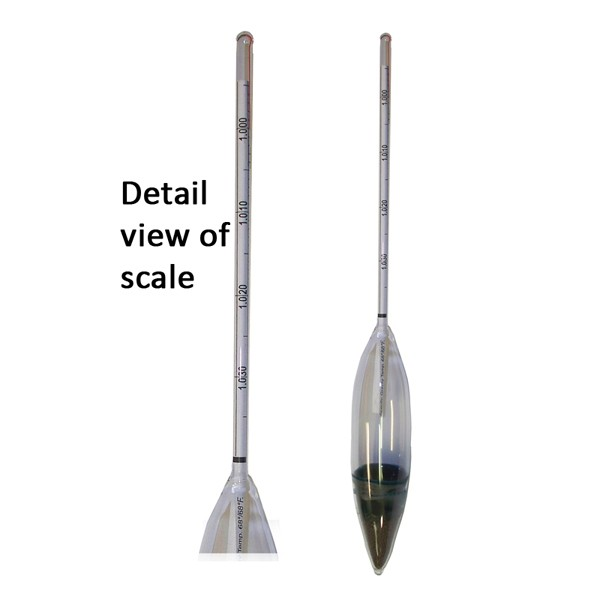
\includegraphics{Hydrometer151H.jpg}
	\caption{Hydrometer 151H. The specific gravity (relative density) of a liquid can be measured using a hydrometer. Hydrometers consist of a bulb attached to a stalk of constant cross-sectional area, as shown in the diagram to the right. The stalk of the hydrometer is pre-marked with graduations to facilitate measurement of the soil suspension, via Archimedes Principle.}
	\label{fig:Hydrometer151H}
\end{marginfigure}

Since the floating hydrometer is in static equilibrium, the downward gravitational force acting upon it must exactly balance the upward buoyancy force. The gravitational force acting on the hydrometer is simply its weight, mg. From the Archimedes buoyancy principle, the buoyancy force acting on the hydrometer is equal to the weight of liquid displaced. This weight is equal to the mass of liquid displaced multiplied by $\rho_\mathrm{ref}$ and the acceleration due to gravity. Thus, the force, $V\rho_{ref}$g\, where V is volume of displaced water, $\rho_{ref}$ is the density of the reference fluid, usually water:  $mg = V\rho_\mathrm{ref}g$, or by canceling the g, 

\begin{equation}\label{eq:massdisplaced}
m = \rho_\mathrm{ref} V,
\end{equation}

and as we'll see below, this can be rearranged to \sidenote{not rearranged... needs to be fixed}

\begin{equation}\label{eq:archmidies}
m = \rho_\mathrm{ref} V,
\end{equation}

Let's describe a comparison of two separate fluids to begin with as shown in Figure \ref{fig:Hydro}, where we can measure the displacement of they hydrometer's depth, where we can evaluate the differences in the relative densities: 

\begin{equation}
RD_{new/ref} = \rho_{new}/\rho{ref}
\end{equation}

\noindent where $\rho_{ref}$ is the known density (mass per unit volume) of the reference liquid (typically water);
$\rho_{new}$ is the unknown density of the new (green) liquid;
$RD_{new/ref}$ is the relative density of the new liquid with respect to the reference;

As the hydrometer is then floated in a liquid of unknown density, $\rho_{new}$, as shown in green in Figure \ref{fig:Hydro}. The change in displacement, $\Delta$x, is noted. In the example depicted, the hydrometer has dropped slightly in the green liquid; hence its density is lower than that of the reference liquid. It is, of course, necessary that the hydrometer floats in both liquids. In accordance with the way in which hydrometers are usually graduated, $\Delta$x is here taken to be negative if the displacement line rises on the stalk of the hydrometer, and positive if it falls. In the example depicted, $\Delta$x is negative.

\begin{marginfigure}
		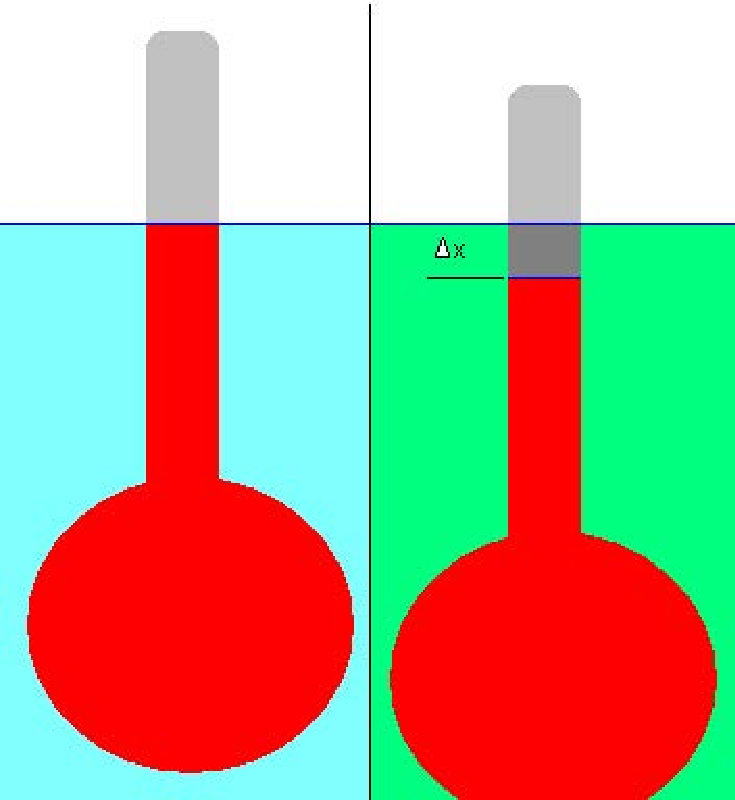
\includegraphics{Hydro.pdf}
	\caption{How does a hydrometer work? First the hydrometer is floated in the reference liquid (shown in light blue), and the displacement (the level of the liquid on the stalk) is marked (blue line). The reference could be any liquid, but in practice it is usually water. }
	\label{fig:Hydro}
\end{marginfigure}

We can modify Equation \ref{eq:archmidies}, by noting that the volume (V) displaced (the red in the figure) has been changed by the displaced volume A$\Delta$x, where A is the cross sectional area of the shaft. Thus, the mass of the hydrometer is 

\begin{equation}\label{eq:hydrometer}
m = \rho_\mathrm{new} (V - A \Delta x),
\end{equation}

\noindent By combining \ref{eq:massdisplaced} and \ref{eq:hydrometer}, we obtain

\begin{equation}\label{eq:RD1}
RD_{\mathrm{new/ref}} = \frac{\rho_\mathrm{new}}{\rho_\mathrm{ref}} = \frac{V}{V - A \Delta x}
\end{equation}

\noindent By re-arranging Equation \ref{eq:massdisplaced}, $V = m/\rho_{ref}$. We can substitute $m/\rho_\mathrm{ref}$ for V into into Eq. \ref{eq:RD1}:

\begin{equation}\label{eq:RD2}
RD_{\mathrm{new/ref}} = \frac{\rho_\mathrm{new}}{\rho_\mathrm{ref}} = \frac{m/\rho_\mathrm{ref}}{m/\rho_\mathrm{ref} - A \Delta x} = \frac{1}{1 - \frac{A \Delta x}{m} \rho_\mathrm{ref}}
\end{equation}

This equation allows the relative density to be calculated from the change in displacement, the known density of the reference liquid, and the known properties of the hydrometer. If $\Delta$x is small then, as a first-order approximation of the geometric series equation \ref{eq:RD2} can be written as:

\begin{equation}\label{eq:RD3}
RD_\mathrm{new/ref} \approx 1 + \frac{A \Delta x}{m} \rho_\mathrm{ref}
\end{equation}

Finally, Equation \ref{eq:RD3} describes how small $\Delta$x, changes in displacement, are approximately proportional to changes in relative density.

%\subsection{Calibrating a Hydrometer -- to be developed}

%Letting $\rho_s$ represent the suspension density, $\rho_f$ the density of fluid, and $\rho_{particle}$ the particle density, all in grams per liter, we have the equation, $\rho_s = \rho_f + (c/1000)(1 - \rho_f/\rho_{particle})$.  Although the buoyant force on a hydrometer is determined directly by the suspension density, r, hydrometer scales can be calibrated in terms of c for particular values of $\rho_l$ and $\rho_s$.  The large size of hydrometer bulb necessary to give adequate sensitivity reduces the depth discrimination of the instrument, but this limitation can be overcome by a simple correction \citep{day1965particle}.

\subsection{ASTM 422D Standard Test Method -- Hydrometer}

The methods to analyze particle distribution has been codified -- in what are compiled by ASTM International -- methods. In this case, the ASTM method 422D, Bouyoucos hydrometer method, was written to analyze particle size in soils or texture \citep{standard2007d422}. The Bouyoucos hydrometer method is somewhat less accurate than the pipet method, but is easier to perform.  The theory of the hydrometer method is similar to that of the pipet method except for the manner of determining the concentration of solids in suspension.  

For the hydrometer reading, the equation for particle size is relative to the effective depth of the hydrometer, in contrast to the distance that particles flow, where

$18 h = 30 l$

$l = 18h/30 = 0.6h$ or $h = 30l/18 = 1.67l$. Unfortunately, I have found no description of how this conversation has been calculated from first principles. For the 151H the effective depth is calculated as $l = 16.295 - 0.2645* R_c$,

However, the method makes a big deal of converting the Hydrometer reading, $R_c$ to the effective depth, that is used in Equation \ref{eq:effectivedepth}.

\begin{equation}\label{eq:effectivedepth}
\texttt{Effective Depth} = 16.295 - 0.1645*Rm
\end{equation}

For analysis of the particle distribution, we calculate the diameter of the particles that remain in suspension, where $d_t < d_0$,  

\begin{equation}
d_e = \sqrt{\frac{30 \eta l}{980 (GS_p - GS_f)* t}}
\end{equation}

\noindent where $d_e$ is the \emph{effective} or \emph{equivalent} settling diameter in mm, 
$\eta$ is the fluid viscosity,
l is effective depth,
$GS_p$ is the specific gravity of soil particles,
$GS_f$ is the specific gravity of fluid, and
$t$ is time of the observation.

In addition, we calculate the proportion of the particles that remain in suspension, which is often called \% Finer, or PF. In other words, the percentage of soil remaining in suspect at the level at which the hydrometer is measuring the density of the suspension may be calculated as follows:

\begin{equation}
PF = [(100,000/M_s)[m|5]P5 \frac{GS_p}{GS_p - GS_w}](R_c - GS_w)
\end{equation}

\noindent where $M_s$ is the soil weight and $GS_p$ is the ratio of the density of soil particles to the density of a reference substance; equivalently, it is the ratio of the mass of a substance to the mass of a reference substance for the same given volume. And $GS_w$ is the specific gravity of water.\sidenote{According to D422-63, using the value of one is appropriate.} $R_c$ is the hydrometer reading after the composite correction applied.\sidenote{The parameter $[m|5]P5$ is note described in the method -- so at this point, I am ignoring the term, which leaves one with an uncomfortable feeling.}

%\subsection{ASTM XXX Standard Test Method -- Pipet }

\subsection{Correction Factors to Consider}

The following are parameters that might influence the results of the hydrometer test and thus, we use various methods to pre-treat soils or measure to correct for these sources of bias. When correction factors are required, the calculations can become confusing.	 But we'll try to lead ourselves through this thicket without too many wrong-turns. 

\begin{description}
	\item[Temperature and Viscosity] Water temperate influences the viscosity of water, such that colder temperatures increase viscosity which increases the resistance force and reduced the terminal velocity of particles. The viscosity can be corrected for temperature.
	\item[Temperature and Density] The density of water is highest at 4.94 degrees C. As temperatures warm, the density of water decreases. As water density decreases, the suspension density $\rho_s$ decreases, thus the particle size distribution is not accurate without a correction. 
	\item[Soil Weight and Hygroscopic Water] Soil is composed of many components, including minerals, water, organic matter, air, etc. But to calculate the soil particle analysis, we need to account for the water in soil. We can do this by measuring the soil moisture content and correct the mass contributed by water from the soil tested.
	\item[Aggregated Soil Particles] Soil particles need to be dispersed, but there is no perfect way to accomplish this. Complete dispersion requires both mechanical and chemical assistance. Mechanical stirring overcomes weaker binding forces in large aggregates, but chemical agents are also necessary, especially to deflocculate clays. Polyvalent cations (normally \ce{Ca+2} and \ce{Al+3}) flocculate clays by forming interparticle, electrostatic links. Chemical dispersing agents (such as sodium hexametaphosphate) are effective in dispersing these clay bundles because:
	
	\begin{itemize}
		\item The sodium monovalent cation (\ce{Na+}) replaces polyvalent cations adsorbed on clays, breaking the interparticle linkage. The displaced polyvalent cations form insoluble complexes with phosphorus that prevents re-establishment of floccules.
		\item The adsorption of sodium, a highly hydrated cation, inducing the hydration of clays. This condition diminishes the binding strength between clay and cation which raises a clay particle's electronegativity and, hence, their repulsion from other clays.
	\end{itemize}
	
The mixture of dispersed soil particles in water is called a suspension. Once a true suspension state has been achieved, differential settling rates can be used to distinguish particle size distribution.
	
	\item Hydrometers are designed to be read from the bottom of the meniscus. However, in a soil suspension, the water is cloudy and we it's impossible to see through the meniscus. Therefore, we read the scale at the top of the meniscus and apply a correction factor. Without this correction factor, the analysis will be incorrect. 
\end{description}

\section{A Simplified Example}

It's generally tough to sort out scientific methods if you can't figure out what the end goal is. For this section, I am giving you an example of some calculations that might be done after the data have been collected.


\subsection{Determining Soil Amount}

After collecting and homogenizing the soil, we allow the soil to air-dry. Then, we passed the sample through the No. 10 sieve, what passes through the No. 10 sieve is particles less than 2 mm. This is considered soil, the rest are gravel or larger rocks. After weighing the percentage of soil that passed through the sieve, we calculated the percent passing through. 

When we report the data, we need to report it as a function of oven-dried soil. However, we don't want to used oven-dried soil for the sedimentation process. Thus, we need to know the difference between the oven-dried and air-dried soil. If the soil is mostly sand, we will need about 100 grams of oven-dried soil and if the soil is a silt or clay soil, we will only need 50 grams of oven-dried soil. 

Again, since we use air-dried soil, we have to correct for the moisture in the soil and use more soil than the 100 or 50 grams as specified above. We figured out that 53.3 grams of air-dried soil equals 50 grams of oven-dried soil, so our sample will have 53.3 grams of air-dried soil, but will be calculated as 50 grams.

\subsection{Observed Results}


We then weighed out 53.3 grams of air-dried soil and let it soak in sodium hexametaphosphate over night. Then we put the soil in 1000 l cylinders and vigorously mix the sample. We started the timer as we stopped mixing and took hydrometer and temperature readings at pre-selected times. 

Using a simple approach where the suspension density is measured several times after mixing, we might observe the following values:

% latex table generated in R 3.3.1 by xtable 1.8-2 package
% Fri Aug 12 22:35:03 2016
\begin{table}[ht]
\centering
\begin{tabular}{rrr}
  \hline
Elapsed Time & Hydrometer Reading & Temperature \\ 
  \hline
0.5 & 1.018 & 23 \\ 
  2.0 & 1.016 & 23 \\ 
  5.0 & 1.012 & 23 \\ 
  15.0 & 1.008 & 23 \\ 
  30.0 & 1.007 & 23 \\ 
  60.0 & 1.006 & 23 \\ 
  120.0 & 1.005 & 23 \\ 
  480.0 & 1.004 & 23 \\ 
  1440.0 & 1.003 & 23 \\ 
   \hline
\end{tabular}
\end{table}
\subsection{Calculating Particle Sizes}

\subsection{Simplest Calculation Method}

\begin{enumerate}
	\item (Clay + silt)\% = (($R_{40s}$ - $Rb_{40s}$)/$W_e$) x 100 
	\item Clay\% = (($R_{8h}$ - $Rb_{8h}$)/$W_e$) x 100 
	\item Silt\% = (Clay + silt)\% - Clay\%

	\item Sand\% = 100 -(($Rb_{40s}$ - $Rb_{40s}$) /$W_e$)*100
	\item Clay\% = ($R_{8h}$ - $Rb_{8h}$) / $W_e$)*100
	\item Silt\% = 100 - Sand\% - Clay\%

\noindent where $R_{40s}$ is the first hydrometer reading at 40s, 
$R_{8h}$ is the hydrometer reading at 8h,
$Rb_{40s}$ and $Rb_{8h}$ are the hydrometer reading of the blank cylinder without soil, and $W_e$ is the weight of soil in the cylinder.

	\item For temperature correction, add or subtract 0.36 g/L for each degree above or below 20$^\circ$C, respectively.
\end{enumerate}

\begin{Schunk}
\begin{Soutput}
[1] 0.074562997 0.037282114 0.023580057 0.013614402 0.009626915 0.006807313 0.004813537 0.002406788
[9] 0.001389571
\end{Soutput}
\begin{Soutput}
[1] 57.818182 51.393939 38.545455 25.696970 22.484848 19.272727 16.060606 12.848485  9.636364
\end{Soutput}
\end{Schunk}


\subsection{Classifying Soil Texture}

After determining the particle sizes, we can ``bin'' or categorize the particle sizes as percentages of sand, silt, and clay. 

\begin{figure}
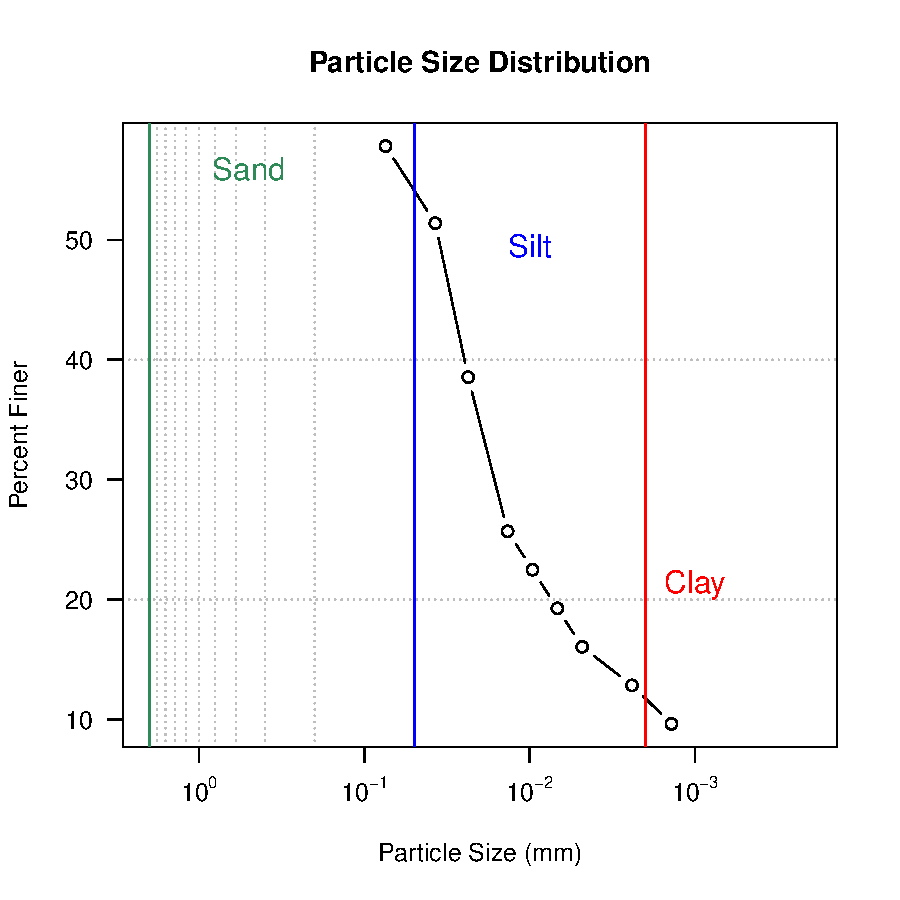
\includegraphics{Soil_Texture_Analysis_160528-simplifiedgraph}
\caption{Particle Size versus Percent Finer remaining in suspension.}
\label{fig.De_vs_PF}
\end{figure}

Using the figure, we estimated the following size classes. Obviously, it would be nice to do a better job than eye-balling the classes, but that will come later in the handout!

\begin{table}

		\begin{tabular}{lr}\hline
Size Class 	&		Percent		\\ \hline\hline
Sand				& 	55\% \\
Silt				&   33\% \\
Clay				& 	12\% \\ \hline		
		\end{tabular}
	\caption{Soil Texture -- Estimated from Figure \ref{fig.De_vs_PF}. Remember, these values should sum to 100\%!}
	\label{tab:SoilTexture}
\end{table}

Finally, we can determine what type of soil we have based on the size-class distribution, which is a sandy loam. 


\begin{figure*}
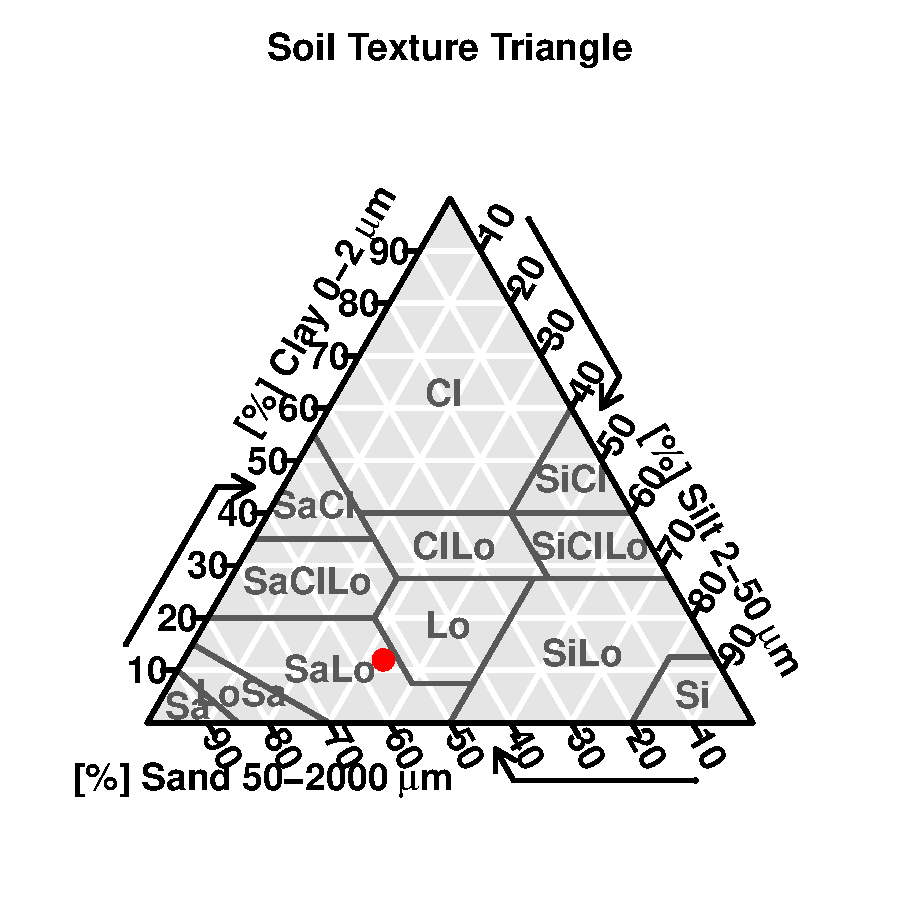
\includegraphics{Soil_Texture_Analysis_160528-TTPlot}
\caption{Results of our texture analysis. Note the small dot in the SaLo (sandy-loam) texture class.}
\label{fig.simplifiedfig}
\end{figure*}



\clearpage
\section{Materials and Procedures}

\subsection{Materials for Hydrometer Method}
\begin{enumerate*}
	\item Sieve No. 10 and No. 200.
	\item 250-ml and 400-ml beakers
	\item Hot plate
	\item Soil tins
	\item Drying oven
	\item Milkshake Mixer and Dispersion Cup (metal milkshake cup)	
	\item 151H Hydrometer
	\item 1 L Sedimentation Cylinder and No. 13 stopper 
	\item Stopwatch
	\item Balance sensitive to 0.01 g for weighing the material passing sieves.
\end{enumerate*}

\section{Reagents}
\begin{enumerate*}
	\item Hydrogen peroxide, 30\%.
	\item Hydrochloric acid, 1N.
	\item Sodium hexametaphosphate
\end{enumerate*}

\section{Procedure}

Before beginning, we need to organize the procedures by day, since we can't complete the analysis during a single lab period.

\begin{description}
	\item[Session 1:] Air dry 200 grams of soil (could require more than one day);
	\item[Session 2:] Pass air-dry soils through No. 10 sieve; dry sub-sample for moisture content; 
	\item[Session 3:] Calculate and weigh $SW_e$ for pretreatment and/or dispersion; 
	\item[Session 4:] Conduct hydrometer measurements; and
	\item[Session 5:] Complete hydrometer readings and data entry.
\end{description}

\subsection{Air-Dried Soil}

After collecting a soil, we allow them to air dry by putting them in a tin or beaker and let them equalibrate with the laboratory for 24 or more hours. If the soils are very wet, this may take several days. 

\subsection{Determining Proportion of Soil Passing No. 10 Sieve}

Soils are defined as particles that are less than 2 mm. Thus, we begin by removing the gravel, particles that exceed the sand-sized particles, >2.0 mm. But these particles influence the soil texture, so we will quantify the contribution of particles that exceed 2 mm. 

We can do this by analyzing the soil that can pass through the No. 10 sieve, which has a mesh size of 2 mm.  

\begin{enumerate}
	\item Homogenize the soil by removing it from the bag and mix thoroughly;
	\item Weigh out approximately 65 g of silt or clay soils or 120 g of a sandy soil, record the value in Box 10. 
	\item Prepare soil with air-drying and pulverizing to pass a No. 10 mesh sieve (< 2 mm)-- pick out the rocks and use a mortar and pestle to break up the soil so that it all passes through the sieve. 
	\item Weigh the soil that passed through the sieve and record the weight in Box 11.
\end{enumerate}
  
\subsection{Measuring and Correcting for Soil Water Content}

We will use air-dried soil for our test. However, even air-dried soil contains water. This moisture is associated with clay particles, salts, and organic matter and is often referred to as hygroscopic water. To calculate the soil moisture content, we weigh the soil before and after oven drying the soil at 110$^\circ$ C. Once we determine the moisture content, we can use the moisture content to correct for the water in the air-dried soil. Because this method relies on the change in soil mass, the water content is often referred to as gravimeter water content as opposed to a volumetric water content.

This temperature is somewhat arbitrary, and clay minerals in particular may contain 10-15\% water (dry basis) at 400$^\circ$ C (Gardner 1986).  As temperature increases, first water in soil pores evaporates, then water adsorbed to mineral surfaces, followed by water between lattice layers and that which forms part of the mineral lattice itself.  The exact quantities and patterns of release in a hetergeneous mixture like soil depends on the particular mix of minerals making up a sample.  Water adsorbed to organic components (as well as other volatile organic substances) will also evaporate over a range of temperatures.  The key point is to specify the temperature used when reporting moisture data.

To determine the hygroscopic water content,

\begin{enumerate}
	\item Weigh and record the weight of a soil tin (Appendix A, Box 13) and the tin \# (Appendix A, Box 12);
	\item Remove a 10-15 gram sub-sample from the air-dried soil that passed through the No. 10 sieve, put the sub-sample into the pre-weighed soil tin and record the weight (Appendix, Box 14);
	\item Dry the sample in a drying oven set at 110 $^\circ$ C for approximately 24 hours;
	\item Allow the tins to cool and record the oven-dried weight (Appendix, Box 15). 
\end{enumerate}

We calculate the  hygroscopic moisture content we subtract the mass of oven-dried sample and the air-dried mass before drying, usually less than one, unless there is no hygroscopic moisture, then is is one. Use the following equation to calculate the water content

\begin{equation}
\texttt{Moisture}_H = (\texttt{air-dry mass w/tin} - \texttt{oven-dried mass w/tin})/(\texttt{air-dried mass} - \texttt{tin mass})
\end{equation}

$Moisture_H$ can be calculated using R code developed for this SOP. See Appendix B for a user guide for the program. 

\subsection{Calculating Soil Sample Mass}

We then calculate the ``Total Sample Represented'' in the hydrometer test as the mass of soil in hydrometer test as the oven dry mass used by the percent passed through 2 mm sieve and multiply by 100.

We will analyze air dried soil -- that has passed through a No. 10 sieve. 


\begin{equation}
W = oven dry mass * percent passing 2mm sieve * 100
\end{equation}

\begin{equation}
WB = \frac{M_{air}*10000}{Per_{No.10} * (100 + Moisture_H)}
\end{equation}

But since the sample has hygroscopic water, we will use the correction factor above to weigh a ``oven-dried equivalent'', $DW_e$. 

If the soils are coarse textured (>70\% sand), will will use $DW_e$ of 100 g, otherwise 50 g is sufficient.

Since air dried soil contains water, the soil sample used will weigh slightly more than 50g or 100 g for sandy soils where $DW_e = DW_{air} * (1 + DW_c)$\sidenote{I need to check this!}, thus we can re-arrange the equation to determine the amount of air-dried soil to use for our test:

\begin{equation}
DW_{air} = 50/(1+DW_c)
\end{equation}

and for sandy soils,

\begin{equation}
DW_{air} = 100/(1+DW_c)
\end{equation}

\subsection{Pre-Treatment}

Soils should be pre-treatmented for soil high in organic matter \ldots

\begin{enumerate}
	\item Transfer 50 or 100 grams of dry weight equivalent ($DW_e$) grams of soil to a 400-ml glass beaker.
	
	\item Removal of carbonates: Add 50 mL DI water and sufficient 1 M \ce{HCl} to reduce the soil pH to between 3.0 and 4.0. Stir and allow to equilibrate 10 minutes until there is no effervescence.

	\item Removal of organic matter: Carefully add 10 ml\sidenote{may need the previous treatment to wet and acidify the soil before this is done. Not clear.} of 30\% hydrogen peroxide (\ce{H2O2}), a few milliliters at a time, allowing effervescence to subside before adding more, until no more frothing occurs. If necessary, make the suspension acidic to litmus paper with a few drops of 1N HCl.  Oxidation with \ce{H2O2} requires an acidic medium. When frothing subsides heat to 90 $^\circ$C and add \ce{H2O2} until frothing subsides. Rinse down walls of beaker and continue heating until no excess \ce{H2O2} is consumed.

	\item Removal of iron oxides \citep[pp. 574-576]{kunze1986pretreatment}: Add 150 mL of citrate-bicarbonate buffer to sample in beaker. Add 3 g of sodium hydrosulfite (\ce{Na2S2O3}) gradually as samples may froth.  Place in water bath at 80$^\circ$C for 20 minutes.  Place the blender cup on electrical mixer and stir for 10 minutes.

	\item Removal of soluble salts: Place soil in centrifuge tube and add 100 mL water and centrifuge for 10 min at 1500 rpm until supernatant is clear.  If the centrifuge is not clear, repeat the process until it is clear.

\end{enumerate}
 
\subsection{Dispersing Soil Sample}

\begin{enumerate}
	\item Using the datasheet and the R function (\texttt{SoilEquiv()}) or web app (http://) to calculate $DW_e$;
	\item Weigh approximately $DW_e$g of soil (From Box 18) into the dispersion cup and record to the nearest 0.1gram (Box 6). 
	\item Record the dispersion cup number (Box 6).
	\item Add 125 mL of sodium hexametaphoshate (40 g/L). Stir so the slurry is thoroughly wetted. Cover and allow to soak for at least 16 hours. 
	\item Add distilled water up to the first ``indentation'' of the dispersion cup.
	\item Attach the dispersion cup to the mixer; mix 5 minutes for sandy soils, 15 minutes for fine-textured soils.
	
\end{enumerate}

\subsection{Conducting Hydrometer Tests}

\begin{enumerate}

	\item Make up a blank cylinder with 125 mL of sodium hexa-metaphosphate and add distilled water to the 1000 mL mark.  Record the blank hydrometer reading and temperature. If the reading is above 0 (zero) on the hydrometer scale (in other words, if the zero mark is below the surface), record the blank correction as a negative number.  Read at the top of the meniscus.
	
	\item Transfer soil suspension to sedimentation cylinder; use distilled water from squirt bottle to get all of sample from mixing cup.

	\item Fill cylinder to 1000-mL mark with distilled water.

	\item Cover the cylinder with a stopper (No. 13) and invert the cylinder 180 degrees for a full minute, where the cylinder should be turned upside-down and back should take 2 seconds. You may need to vigorously mix the cylinder for the first two turns to loose the soil at the bottom.
	
	\item After the minute of inverting, begin timing.  While slowing spinning the hydrometer remove air bubbles, carefully lower the hydrometer into suspension after 20s; record the hydrometer reading at 40 seconds. Remove the hydrometer and rinse the hydrometer between each reading. 
	
	\item This 40-second reading should be \textbf{repeated to obtain 3 accurate} after repeating the inversion process.\sidenote{Because the suspension is opaque, read the hydrometer at the top of the meniscus rather than at the bottom. There is a correction for this!}

	\item After final 40-second reading, remove hydrometer, carefully lower a thermometer into the suspension and record the temperature (degrees C).  Mixing raises temperature by 3-5$^\circ$C, so it is important to record the temperature for both hydrometer readings (See Table \ref{tab:ReadingTimes}).
	
		\item The hydrometer must be removed and rinsed and dried after each reading. If this is not followed, the hydrometer will be accumulate particles on the glass walls and become increasingly inaccurate. 

	\item Take a hydrometer reading at the following times:
	
		\begin{table}
		\begin{tabular}{lrr}\hline
Obs. & Soil Reading Times & Temperature Reading		& Blank Hydrometer \& Temperature \\ \hline\hline	
0		& Before Inverting (0 seconds)		&	 X	&		X		\\
1		& 40 seconds (Repeat twice) 			&	 		&			  \\
2		&	2.0 minutes 										&			&       \\
3		&	5.0 minutes 										&	 X 	&		X   \\
4		&	15 minutes 											&	 		&   	  \\
5	 	& 30 minutes 											&			&				\\
6		& 60 minutes 											&		X	& 	X		\\
%X		& 90 minutes 										&			&				\\
7		& 2	hours													& 	X	& 	X		\\
8		& 3 hours (optional)							&		X	& 	X		\\
9   & 6 or 8 hours (optional)					&		X	& 	X		\\
10		& 24 hours											&		X	&  	X 	\\\hline		
		\end{tabular}
		\caption{Reading times modified from \citet{standard2007d422}. These times can be adjusted, be sure to record the actual times in Boxes 19 and 20.}
		\label{tab:ReadingTimes}
	\end{table}
	
	\item Be sure that the cylinder is back from the edge of the counter and in a location where it won't be disturbed.	
	
\end{enumerate}

\section{Recording the Results}

Record the results in Appendix A, into the following columns: 19, 20, 21, 23. Other columns calculations will be produced with the R code from Appendix B.  

\section{Particle Size Distribution Calculations}

Once the data has been entered in the online form, you can extract the data as a csv file. This csv file can then be called by R to calculate the data automatically, using the following functions. 

\subsection{Importing Data}

Import and check data integrity

\begin{Schunk}
\begin{Sinput}
> #hydrometer = import()
> #head(hydrometer)
> #str(hydrometer)
\end{Sinput}
\end{Schunk}

What should you be looking for?  We want to make sure the data shown are the same as expected. There are several ways to look at the data to determine this. I have shown two ways. 1) Looking at the header (first six observations), then we evaluate the structure of the dataframe.
 
\subsection{Calculating effective diameter, $D_e$}


\subsection{Calculating the Percent Finer, PF}

\subsection{Graphing and Interpreting the Results}


plot(PF ~ De, data=tmp2)

plot(tmp2$De, tmp2$PF, ty='b', las=1, log='x', xaxt='n', xlim=c(2, 0.0002), ylab = "Percent Finer", xlab="Particle Size (mm)", main='Particle Size Distribution', panel.first=abline(v=seq(2, 0, -0.2),h=c(20,40,60,80), lty=3,col="gray"))
ticks <- seq(-5, 0, by=1)
labels <- sapply(ticks, function(i) as.expression(bquote(10^ .(i))))
axis(1, at=c(0.00001, 0.0001, .001, 0.01, 0.1, 1.0), labels=labels)
grid(nx = NULL, ny = 1, col = "lightgray", lty = "dotted",
     lwd = par("lwd"), equilogs = F)

# Minor Grids
n <- n+2 <4
minors <- log10(pretty(10^major.ticks[1:2],n))-major.ticks[1]
minors <- minors[-c(1,n)]
minor.ticks = c(outer(minors,major.ticks,`+`))
minor.ticks <- minor.ticks[minor.ticks > mn & minor.ticks < mx]
axis(ax,at=minor.ticks,tcl=par("tcl")*t.ratio,labels=FALSE)

abline(v=0.002, col='Red'); text(x = .001, y = PF[6], 'Clay', col='red', cex=1.25, pos=3)
abline(v=0.05, col='Blue'); text(x = .01, y = PF[4], 'Silt', col='blue', cex=1.25, pos=1)
abline(v=2.0, col='Green'); text(x = 0.50, y = PF[1], 'Sand', col='green', cex=1.25, pos=1)


%#sand = approx(x, y = NULL, xout, method = "linear", n = 50, yleft, yright, rule = 1, f = 0, ties = mean)

TT.points.in.classes(tri.data = texturetest, class.sys = "USDA.TT") 

\section{Conclusion}



\FloatBarrier 
\begin{fullwidth}
% \renewcommand{\bibfont}{\small}
\bibliography{../../../CA_Limnology/CA_limnology}

\bibliographystyle{cbe}

\medskip
\noindent \textbf{Other Citations of Interest:} 

Wilde, S.A., R.B. Corey, J.G. Iyer, and G.K. Voigt.  1979.  Soil and Plant Analysis for Tree Culture.  Oxford and IBH Publishing Co., New Delhi.  Pp. 12-13.

Anderson, J.M., and J.S. Ingram, eds.  1993.  Tropical Soil Biology and Fertility:  A Handbook of Methods. 2nd ed.  CAB International, Wallingford, UK.  P. 93-94.

\end{fullwidth}


\newpage
\thispagestyle{empty}
\section{Appendix A. Data Sheet}
\begin{fullwidth}
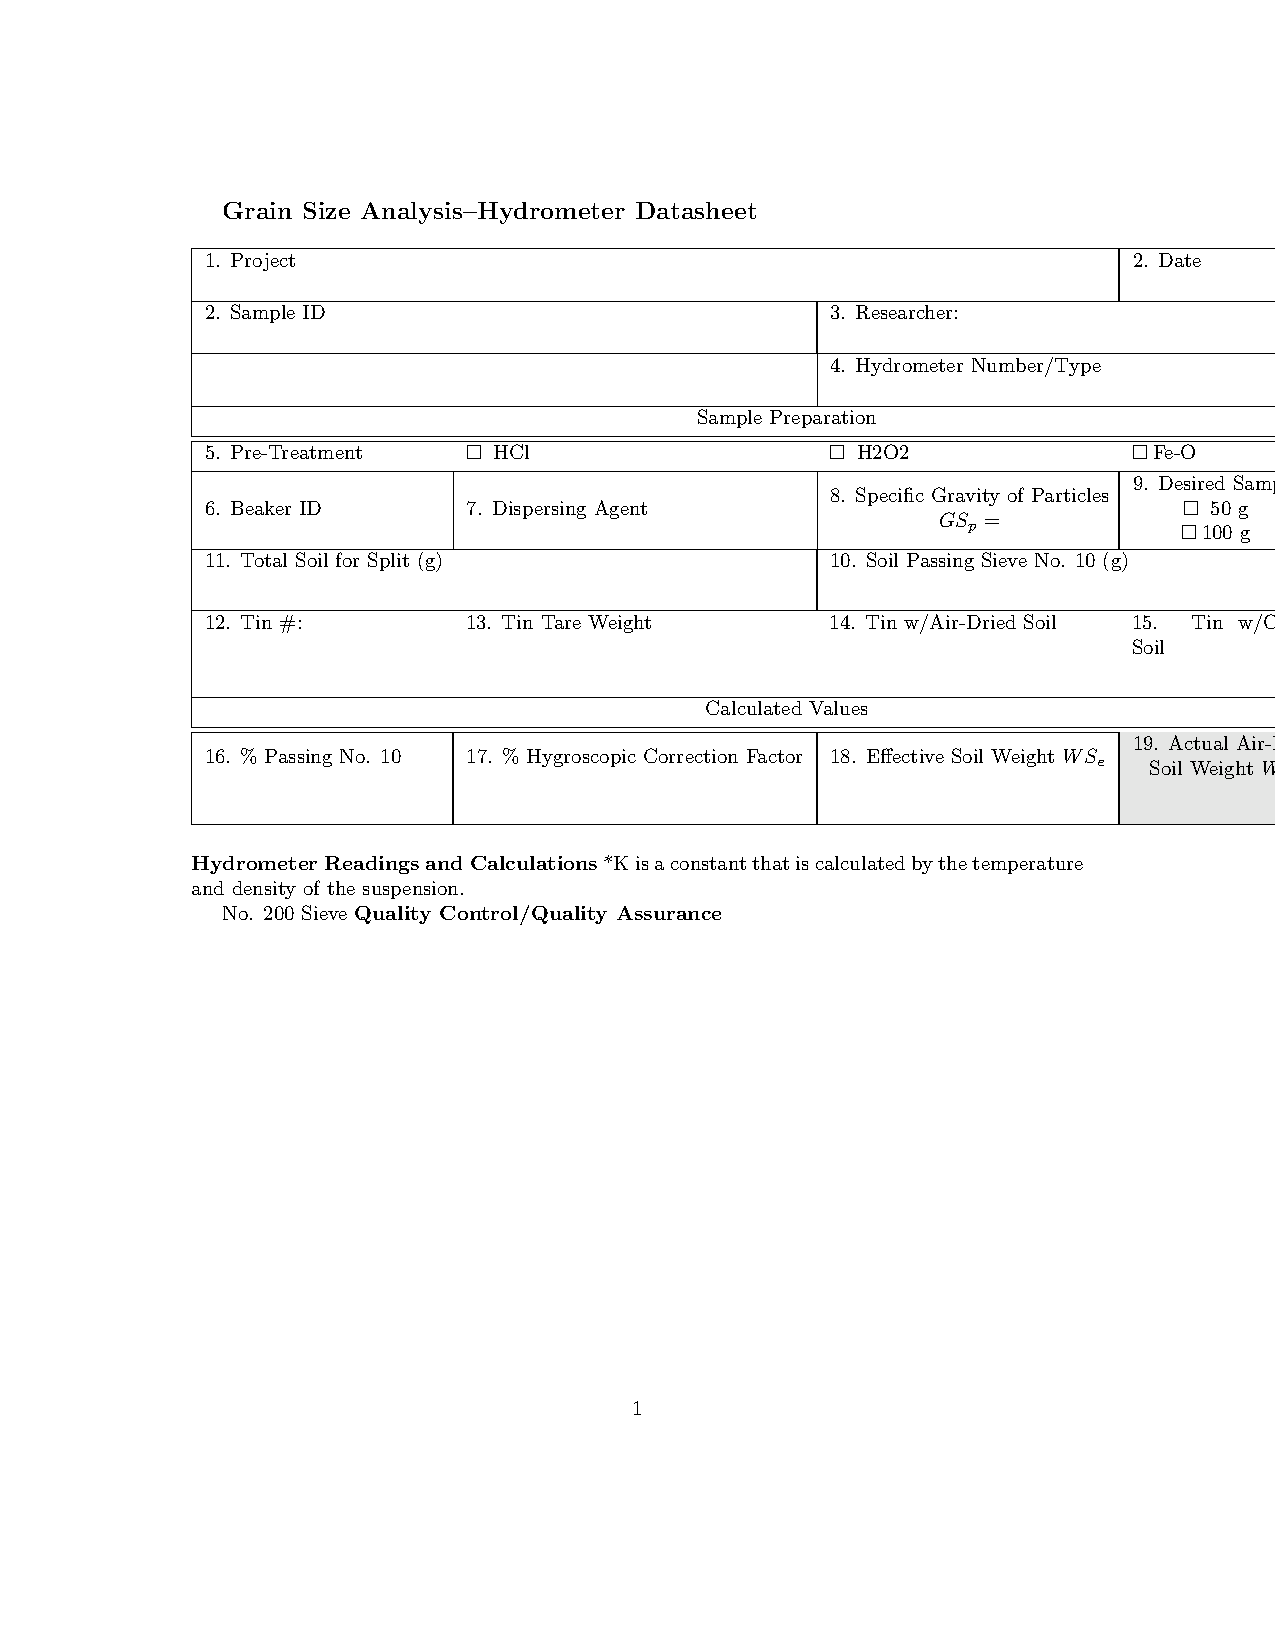
\includepdf[pages=-]{DataSheetv2}
\end{fullwidth}


\newpage
\section{Appendix B: R code to calculate parameters for the SOP}

\subsection{Percent Passing Through No. 10 Sieve}

Using the function below, we can calculate the amount of soil that passed through Sieve No. 10. Once the function is call, record the results into Box 16. 

\begin{Schunk}
\begin{Sinput}
 PassNo10 = function(MassPassed,Total){
   PercentPassed = MassPassed/Total * 100
   cat("Enter", round(PercentPassed, 1), "into Box 16")
 }
\end{Sinput}
\end{Schunk}

The syntax of the function requires two parameters, mass of soil passed (Box 11) and total soil used (Box 10), PassNo10(Mass of Soil Passed, Total Soil Used). 

For example, if we have the mass of the soil that passed through the sieve 122 grams and we had a total to start with of 133 grams.

\begin{Schunk}
\begin{Sinput}
 PassNo10(122, 133)
\end{Sinput}
\begin{Soutput}
Enter 91.7 into Box 16
\end{Soutput}
\end{Schunk}

\subsection{Calculating Soil Mass for Analysis}

The following function can be used to calculate the ...

\begin{Schunk}
\begin{Sinput}
 # Function to Calculate Ws 
 SoilEquiv = function(tin, airdry, ovendry, tinmass, desiredmass = 50){
 hygro = round(ovendry/airdry, 2)
 wd = (airdry - ovendry)/(ovendry-tinmass)
 WS_e = round(desiredmass * (1 + wd), 2)
 output = data.frame(
   Parameter = c("Tin ID", "Tin Tare Weight", "Mass of air-dried soil", 
       "Mass of oven-dried soil", "Hygroscopic Correction Factor", 
       "Desired Oven-dried Soil", "Effective Soil Weight (WSe)"),
   Value = c(tin, tinmass, airdry, ovendry, hygro, desiredmass, WS_e),
   Box = c(12, 13, 14, 15, 17, 9, 18))
 print(output)
 }
\end{Sinput}
\end{Schunk}

The function (SoilEquiv) requires four parameters to run provide the output, the mass of soil to be used for the hydrometer test. This mass is the air-dried soil to be used but is equivalent to the desired oven-dried soil, is based on the hygroscopic water methods. 

The function's syntax is as follows: SoilEquiv(Tin \#, Air-Dried Mass, Oven-Dried Mass, Tin Tare, Desired Oven-Dried Soil)

Below is an example, where the $tin number = 4$, $airdry = 27.4$, $ovendry = 25.6$, $tinmass = 12.3$, $desiredmass = 50$ and as used in R: 

\begin{Schunk}
\begin{Sinput}
 SoilEquiv(4, 27.4, 25.6, 12.3, 50)
\end{Sinput}
\begin{Soutput}
                      Parameter Value Box
1                        Tin ID  4.00  12
2               Tin Tare Weight 12.30  13
3        Mass of air-dried soil 27.40  14
4       Mass of oven-dried soil 25.60  15
5 Hygroscopic Correction Factor  0.93  17
6       Desired Oven-dried Soil 50.00   9
7   Effective Soil Weight (WSe) 56.77  18
\end{Soutput}
\end{Schunk}


\subsection{Hydrometer Correction Factor}

Correcting for the meniscus, we use our ``blank'' hydrometer readings to calculate the composite correction factor, CCF. 

\begin{equation}
R_c = R_a - (R_b - 1)
\end{equation}

The equation is implemented in the De function below...



\subsection{Effective Depth}

We have two hydrometer types in the lab -- and the formula to calcutate the effective depth varies based on which hydrometer we use. 

\begin{equation}
\texttt{Effective Depth} = XXX
\end{equation}

\begin{table}
		\begin{tabular}{lcl}\hline
Hydrometer Model	& Code for R function  	&	$R = f(R_a)$	\\ \hline\hline
Heavy Liquid			&		``HL''							&	$16.295 - 0.1645 * R_c$\\
151H Hydrometer		& 	``151H''						& $234.9 + -228.X * R_c$\\ \hline
		\end{tabular}
	\caption{Hydrometer Types and Effective Depth Formula}
	\label{tab:HydrometerTypesAndEffectiveDepthFormula}
\end{table}

Thus, the function syntax is

Hydrometer = ``HL'' or Hydrometer = ``151H''

\subsection{Formatting the Data}

There are two ways to process the data. One, you can analyze the data using a calculator or use excel as a fancy calculator. Either way, we are not using the efficacy of using available software. For our analysis, we will analyze the data using R that is capable of analyzing many samples simultaneously. In order to accomplish this, we need to have the data entered in a consistent format. 

Thus, we have created a spreadsheet or access database? for data entry or shiny apps?

\subsection{Importing data}

importing data into R is not difficult, but there are tricks. The following function, allows the data to be imported into R from a csv file. This function is used to start the analysis. 

\begin{Schunk}
\begin{Sinput}
 import = function(){
 read.csv(file.choose())
 }
\end{Sinput}
\end{Schunk}

\subsection{Calculating the $D_e$ and PF w/K}

Below is the function to calculate the D and PF, where K as a constant is calculated. 

\subsection{Effective Particle Diameter Size, $D_e$}

The formula is 

\begin{equation}
d_e = \sqrt{\frac{30 \eta l}{980 (GS_p - GS_f)* t}}
\end{equation}

Once the data have been inspected for integrity, we can use the following function to calculate the two values of interest: $D_e$ and PF. 

